\documentclass[10pt,twocolumn]{article}

% ---------- packages ----------
\usepackage[T1]{fontenc}
\usepackage[utf8]{inputenc}
\usepackage[margin=1.9cm]{geometry}
\usepackage{amsmath,amssymb}
\usepackage{booktabs}
\usepackage[expansion=false]{microtype}
\usepackage{xcolor}
\usepackage{caption}
\usepackage{pgfplots}
\pgfplotsset{compat=1.17}
\usepackage[colorlinks=true,allcolors=blue!55!black]{hyperref}

\captionsetup{font=small,labelfont=bf}
\setlength{\parindent}{1.1em}
\pagestyle{plain}

% palette
\definecolor{orthogrey}{HTML}{6B7280}
\definecolor{blastblue}{HTML}{2563A6}
\definecolor{plmgreen}{HTML}{1B7F5E}

\title{\vspace{-1.2em}\textbf{\large Cross-species single-cell RNA-seq integration:\\
from one-to-one orthologs to protein-language-model embeddings}}
\author{\normalsize A literature review of primary methods and recent benchmarks}
\date{\normalsize July 2026}

\begin{document}
\twocolumn[
  \begin{@twocolumnfalse}
  \maketitle
  \vspace{-1.0em}
  \begin{center}
  \small
  \begin{tabular}{@{}llll@{}}
  \toprule
  \textbf{Methods surveyed} & \textbf{Span} & \textbf{Benchmarks} & \textbf{Widest divergence} \\
  \midrule
  15 primary tools & 2018--2025 & 3 dedicated & $>$1.5\,Gyr (TranscriptFormer) \\
  \bottomrule
  \end{tabular}
  \end{center}
  \vspace{0.6em}

  \begin{abstract}
  \noindent Comparative single-cell transcriptomics asks whether a cell type in one
  species has a homologue in another, and how its expression program has been
  conserved or rewired. The technical obstacle is that any two species'
  transcriptomes live in different gene coordinate systems. We review the three
  strategies that the field has used to bridge them: (i) subsetting to one-to-one
  orthologs and treating species as a batch, the recipe behind Seurat, LIGER,
  Harmony, Scanorama, BBKNN and the scVI family; (ii) replacing the hard ortholog
  filter with a soft, sequence-homology graph, as in SAMap; and (iii) discarding
  orthology entirely by embedding genes of every species into a common
  protein-language-model space, as in SATURN, UCE and TranscriptFormer. We
  summarise the primary methods papers, the evidence from three recent
  cross-species benchmarks, and the open problems that remain.
  \end{abstract}
  \vspace{0.8em}
  \end{@twocolumnfalse}
]

% =====================================================================
\section{Problem statement}
% =====================================================================
A cell atlas maps the cell types of an organism; a \emph{comparative} atlas asks
which of those types are shared across organisms and which are lineage
innovations. Answering this at single-cell resolution requires placing cells from
two or more species into one representation in which biological cell identity, and
not the species of origin, drives the geometry. The obstacle is fundamental:
transcriptomes are indexed by genes, and gene repertoires diverge. Orthologs are
frequently many-to-many after lineage-specific duplication, lineage-specific genes
have no counterpart at all, and even one-to-one orthologs can be co-opted into new
expression programs. Integration methods differ chiefly in \emph{how much} of this
gene-level divergence they try to model, and that choice defines the three
generations of tools reviewed here (Figure~\ref{fig:timeline}).

The first generation borrowed directly from within-species batch correction: after
restricting both datasets to a shared one-to-one ortholog table, the species label
is treated as just another batch covariate to be removed. This is convenient and,
within mammals ($\sim$90\,Mya divergence), largely defensible, because most genes
still have a clean ortholog. It fails once the ortholog table itself becomes small
or undefined --- between vertebrates and invertebrates, or where no reference
orthology exists. The second and third generations were built to reach those
distances.

% =====================================================================
\section{Ortholog-subsetting methods}
% =====================================================================
\paragraph{Anchor- and factor-based aligners.}
Seurat~v3~\cite{stuart2019} finds correspondences by diagonalized canonical
correlation analysis: it computes shared canonical-correlation vectors over the
common-ortholog matrices, L2-normalises them, and calls mutual nearest neighbours
in that subspace ``anchors,'' which then drive a smooth correction and can transfer
labels across datasets or species. LIGER~\cite{welch2019} instead factorises each
dataset by integrative non-negative matrix factorisation, $X_k \approx (W+V_k)H_k$,
sharing metagene factors $W$ across species while isolating dataset-specific signal
in $V_k$. Harmony~\cite{korsunsky2019} operates post-PCA, iteratively soft-clustering
cells and shifting centroids to maximise batch diversity within each cluster; its
linear correction is fast and sensitive but, like every method in this section,
can only recover signal that survives the ortholog bottleneck. Scanorama~\cite{hie2019}
and BBKNN~\cite{polanski2020} work at the graph level, stitching or rebalancing
nearest-neighbour graphs across batches without an explicit generative model.

\paragraph{Conditional variational autoencoders.}
Deep generative models follow the same subset-then-batch recipe but absorb the
species label into the decoder. scVI~\cite{lopez2018} fits a conditional VAE over
the shared gene set, optimising the evidence lower bound
\begin{equation}
\mathcal{L}(\theta,\phi) = \mathbb{E}_{q_\phi(\mathbf z\mid \mathbf x,s)}
\!\big[\log p_\theta(\mathbf x\mid \mathbf z,s)\big]
- D_{\mathrm{KL}}\!\big(q_\phi(\mathbf z\mid \mathbf x,s)\,\Vert\,p(\mathbf z)\big),
\label{eq:elbo}
\end{equation}
where $s$ is the species/batch indicator. Because $s$ enters only the decoder, the
latent $\mathbf z$ is, in principle, species-invariant. scANVI~\cite{xu2021} extends
Eq.~\eqref{eq:elbo} with a semi-supervised label head, and scArches~\cite{lotfollahi2022}
adds lightweight adapter weights so a new species can be mapped onto a frozen
reference without retraining. scPoli~\cite{dedonno2023} augments the same backbone
with learnable per-sample (or per-species) prototype embeddings, making the
conditioning multi-scale rather than a single one-hot covariate. scGen~\cite{lotfollahi2019}
combines a VAE with explicit latent-space vector arithmetic and is a strong batch
remover in the cross-species benchmarks below. The shared limitation is
Eq.~\eqref{eq:elbo}'s support: every term is defined only on the intersection gene
set, so lineage-specific and rewired genes are invisible by construction.

% ---------- figure ----------
\begin{figure}[t]
\centering
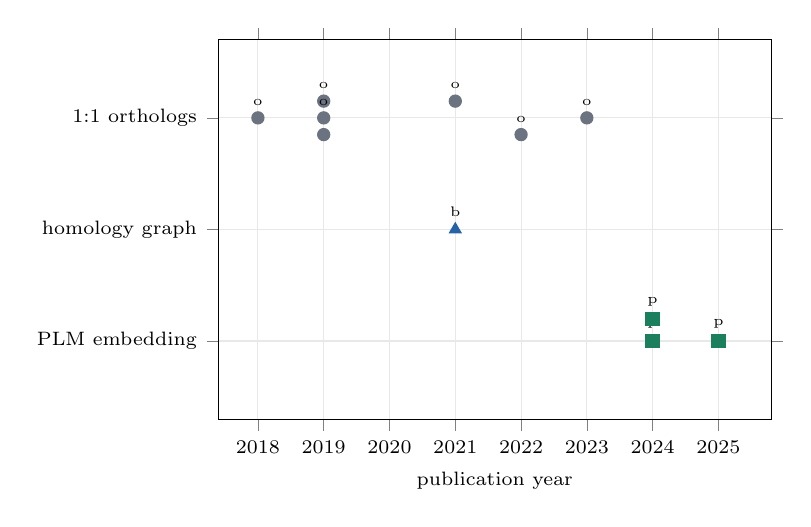
\begin{tikzpicture}
\begin{axis}[
  width=8.6cm, height=6.4cm,
  xmin=2017.4, xmax=2025.8,
  ymin=0.3, ymax=3.7,
  xtick={2018,2019,2020,2021,2022,2023,2024,2025},
  xticklabel style={font=\scriptsize,/pgf/number format/1000 sep=},
  ytick={1,2,3},
  yticklabels={{PLM embedding},{homology graph},{1:1 orthologs}},
  yticklabel style={font=\scriptsize,align=right},
  ylabel style={font=\scriptsize},
  xlabel={publication year}, xlabel style={font=\scriptsize},
  tick align=outside, grid=major, grid style={gray!18},
  scatter/classes={
    o={mark=*,orthogrey},
    b={mark=triangle*,blastblue},
    p={mark=square*,plmgreen}},
]
% 1:1 ortholog tools (y=3)
\addplot[scatter,only marks,mark size=2.2pt,
  scatter src=explicit symbolic,
  nodes near coords*={\pgfplotspointmeta},
  visualization depends on={value \thisrow{lbl}\as\lbl},
  every node near coord/.append style={font=\tiny,anchor=south,yshift=1pt},
  point meta=explicit symbolic]
table[meta=class]{
x    y   class  lbl
2018 3   o      scVI
2019 3.15 o     Seurat
2019 2.85 o     LIGER
2019 3.0 o      Harmony
2021 3.15 o     scANVI
2022 2.85 o     scArches
2023 3.0 o      scPoli
};
% homology-graph (y=2)
\addplot[scatter,only marks,mark size=2.4pt,
  scatter src=explicit symbolic,point meta=explicit symbolic,
  nodes near coords*={\pgfplotspointmeta},
  every node near coord/.append style={font=\tiny,anchor=south,yshift=1pt}]
table[meta=class]{
x    y   class  lbl
2021 2   b      SAMap
};
% PLM embedding (y=1)
\addplot[scatter,only marks,mark size=2.4pt,
  scatter src=explicit symbolic,point meta=explicit symbolic,
  nodes near coords*={\pgfplotspointmeta},
  every node near coord/.append style={font=\tiny,anchor=south,yshift=1pt}]
table[meta=class]{
x    y   class  lbl
2024 1   p      SATURN
2024 1.2 p      UCE
2025 1   p      TranscriptFormer
};
\end{axis}
\end{tikzpicture}
\caption{\textbf{Three generations of cross-species integration.} Primary methods
positioned by publication year and by how they cross the gene-coordinate gap.
Ortholog-subsetting tools (grey) dominate the early field because they double as
batch-correction methods; the sequence-homology graph of SAMap (blue) and the
protein-language-model embedders (green) are more recent and were built to span
$>$400\,Mya divergence, where a one-to-one ortholog table is small or undefined.}
\label{fig:timeline}
\end{figure}

% =====================================================================
\section{Homology-graph methods}
% =====================================================================
SAMap~\cite{tarashansky2021} was the first tool to abandon the hard ortholog filter
without abandoning gene identity. It replaces the fixed one-to-one table with a
soft, BLAST-derived gene-homology weight matrix $\mathbf H$ and refines it
iteratively against the cell-level manifold. Cross-species cell similarity is scored
as
\begin{equation}
M_{ij}=\frac{\langle \mathbf x_i,\mathbf H\mathbf y_j\rangle}
{\lVert \mathbf x_i\rVert\,\lVert \mathbf H\mathbf y_j\rVert},
\label{eq:samap}
\end{equation}
so that a gene in one species can contribute to a cell's profile in another through
any of its sequence homologues --- including paralogs, not only reciprocal best
hits. Building on the self-assembling manifold algorithm, SAMap alternates between
updating $\mathbf H$ and re-embedding cells until mutual cross-species neighbourhoods
stabilise. This made integration across $>$500\,Mya (sponge--planarian--schistosome
--zebrafish) tractable for the first time, and, notably, the authors found many
genes whose expression more closely tracks a paralog than the annotated ortholog,
evidence that paralog substitution in cell-type programs is more common than a
strict ortholog view assumes.

% =====================================================================
\section{Protein-language-model embeddings}
% =====================================================================
The most recent generation removes the orthology call entirely. Instead of matching
genes, it embeds every gene --- from any species --- into a shared space defined by
its protein sequence, using a protein language model such as ESM2.

\paragraph{SATURN.}
SATURN~\cite{rosen2024} takes scRNA-seq counts plus ESM2 protein embeddings for each
species' genes, and learns ``macrogenes'' --- soft clusters of functionally related
proteins --- that provide a common feature basis across datasets with disjoint gene
sets. Cells are then mapped to a joint low-dimensional space using expression coupled
to these protein representations. Because the shared basis is defined by sequence and
not by an ortholog table, SATURN transfers annotations even between evolutionarily
remote species and can flag genes that are co-expressed and functionally related
across species without being orthologs.

\paragraph{Universal Cell Embeddings.}
UCE~\cite{rosen2026} pushes the idea to a self-supervised foundation model: a large
transformer tokenises genes through their ESM2 protein embeddings and is trained,
with no cell-type labels, on a corpus spanning human and seven other species. The
resulting encoder maps any cell --- including cells from species absent from
training --- into a single latent space with no fine-tuning, and was used to build an
Integrated Mega-scale Atlas of tens of millions of cells across eight species. Its
zero-shot, label-free operation is the practical payoff of the protein-space
approach.

\paragraph{TranscriptFormer.}
TranscriptFormer~\cite{transcriptformer2025} is a generative foundation model that
jointly models genes and transcript counts with expression-aware attention, trained
on up to 112\,million cells spanning twelve species and roughly 1.5\,billion years of
evolution. In zero-shot settings it classifies cell types robustly even for species
separated by hundreds of millions of years, and, being generative, it can be prompted
to predict cell-type-specific transcription factors and gene--gene interactions,
extending cross-species integration from alignment toward hypothesis generation.

% =====================================================================
\section{Benchmarks and evaluation}
% =====================================================================
Method proliferation has been matched by three benchmarking efforts of increasing
cross-species scope. The scIB study of Luecken~et~al.~\cite{luecken2022} is not
cross-species per se but set the evaluation template the field reuses: 68
method/preprocessing combinations over 1.2\,M cells and 13 atlas-level tasks, scored
by a weighted combination of batch-removal and biological-conservation metrics. Its
central finding --- that aggressive scaling trades biological conservation for batch
removal --- recurs in every cross-species study.

BENGAL~\cite{song2023} was the first benchmark dedicated to the cross-species
question. It factorised the problem into two orthogonal choices --- how genes are
mapped by homology (four schemes) and which integration algorithm is applied (ten
methods) --- giving 28 strategies across 16 tasks on vertebrate cell types with clear
one-to-one correspondences, and it contributed a conservation metric tailored to
preserving cell-type distinguishability. Its message is that the gene-mapping step is
as consequential as the integration algorithm, a variable the ortholog-subsetting
literature had treated as fixed.

The most recent and most divergent benchmark, Zhong~et~al.~\cite{zhong2025},
evaluated nine methods across 20 species, 4.7\,million cells and eight phyla ---
effectively the whole animal taxonomic hierarchy. Two conclusions stand out. First,
methods that exploit gene \emph{sequence} information (SATURN) best preserved
biological variance across large taxonomic distances, while generative
batch-correction models (e.g.\ scGen) were strongest at species mixing --- the same
conservation-versus-removal tension, now resolved differently by method class.
Second, no single tool dominated: SATURN was the most consistent from cross-genus to
cross-phylum, SAMap was strongest for atlas-level integration beyond the cross-family
level, and conditional-VAE methods remained competitive only within or below the
cross-class range. In short, the right tool is a function of evolutionary distance.

\begin{table}[t]
\centering
\small
\caption{Recommended method class by evolutionary distance, synthesising the
cross-species benchmarks~\cite{song2023,zhong2025}.}
\label{tab:reco}
\begin{tabular}{@{}p{2.55cm}p{2.0cm}p{2.5cm}@{}}
\toprule
\textbf{Divergence} & \textbf{Ortholog table} & \textbf{Best-supported class} \\
\midrule
Intra-mammal ($\lesssim$100\,Mya) & dense 1:1 & conditional VAE / anchor \\
Cross-class / vertebrate & thinning & sequence-aware (SAMap) \\
Cross-phylum ($>$400\,Mya) & sparse/absent & PLM embedding (SATURN/UCE) \\
\bottomrule
\end{tabular}
\end{table}

% =====================================================================
\section{Discussion and open problems}
% =====================================================================
The trajectory of the field is a steady weakening of the orthology assumption: from a
hard one-to-one filter, to a soft sequence-homology graph, to a protein-sequence
embedding in which orthology is never called. Each step widens the reachable
evolutionary distance but also loosens the biological anchor that makes an alignment
interpretable, which is why evaluation has become the central difficulty rather than
an afterthought.

Three problems remain open. First, \emph{ground truth}: cross-species benchmarks rely
on expert-assigned homologous cell types, which are themselves hypotheses, so a method
that ``mixes'' species well may be rewarded for erasing genuine divergence. Second,
\emph{sequence is not expression}: protein-language-model embeddings encode what a
protein \emph{is}, not where or when it is transcribed, so two sequence-similar genes
with divergent regulation can be conflated --- the very paralog-substitution signal
that SAMap exposed. Third, \emph{interpretability at scale}: foundation-model
embeddings deliver zero-shot convenience but make it harder to attribute an alignment
to specific conserved genes, exactly the biological readout comparative studies want.
Progress will likely come from hybrids that keep the protein-space reach of SATURN and
UCE while restoring an explicit, testable gene-level account of what has been
conserved and what has been rewired.

% =====================================================================
\begin{thebibliography}{99}
\small
\bibitem{stuart2019} Stuart T, Butler A, Hoffman P, \emph{et al.}
Comprehensive integration of single-cell data. \emph{Cell} 177:1888--1902 (2019).
\href{https://doi.org/10.1016/j.cell.2019.05.031}{doi:10.1016/j.cell.2019.05.031}.

\bibitem{welch2019} Welch JD, Kozareva V, Ferreira A, \emph{et al.}
Single-cell multi-omic integration compares and contrasts features of brain cell
identity (LIGER). \emph{Cell} 177:1873--1887 (2019).
\href{https://doi.org/10.1016/j.cell.2019.05.006}{doi:10.1016/j.cell.2019.05.006}.

\bibitem{korsunsky2019} Korsunsky I, Millard N, Fan J, \emph{et al.}
Fast, sensitive and accurate integration of single-cell data with Harmony.
\emph{Nat Methods} 16:1289--1296 (2019).
\href{https://doi.org/10.1038/s41592-019-0619-0}{doi:10.1038/s41592-019-0619-0}.

\bibitem{hie2019} Hie B, Bryson B, Berger B.
Efficient integration of heterogeneous single-cell transcriptomes using Scanorama.
\emph{Nat Biotechnol} 37:685--691 (2019).
\href{https://doi.org/10.1038/s41587-019-0113-3}{doi:10.1038/s41587-019-0113-3}.

\bibitem{polanski2020} Pola\'nski K, Young MD, Miao Z, \emph{et al.}
BBKNN: fast batch alignment of single cell transcriptomes.
\emph{Bioinformatics} 36:964--965 (2020).
\href{https://doi.org/10.1093/bioinformatics/btz625}{doi:10.1093/bioinformatics/btz625}.

\bibitem{lopez2018} Lopez R, Regier J, Cole MB, Jordan MI, Yosef N.
Deep generative modeling for single-cell transcriptomics (scVI).
\emph{Nat Methods} 15:1053--1058 (2018).
\href{https://doi.org/10.1038/s41592-018-0229-2}{doi:10.1038/s41592-018-0229-2}.

\bibitem{xu2021} Xu C, Lopez R, Mehlman E, \emph{et al.}
Probabilistic harmonization and annotation of single-cell transcriptomics data with
deep generative models (scANVI). \emph{Mol Syst Biol} 17:e9620 (2021).
\href{https://doi.org/10.15252/msb.20209620}{doi:10.15252/msb.20209620}.

\bibitem{lotfollahi2022} Lotfollahi M, Naghipourfar M, Luecken MD, \emph{et al.}
Mapping single-cell data to reference atlases by transfer learning (scArches).
\emph{Nat Biotechnol} 40:121--130 (2022).
\href{https://doi.org/10.1038/s41587-021-01001-7}{doi:10.1038/s41587-021-01001-7}.

\bibitem{dedonno2023} De Donno C, Hediyeh-Zadeh S, Moinfar AA, \emph{et al.}
Population-level integration of single-cell datasets enables multi-scale analysis
across samples (scPoli). \emph{Nat Methods} 20:1683--1692 (2023).
\href{https://doi.org/10.1038/s41592-023-02035-2}{doi:10.1038/s41592-023-02035-2}.

\bibitem{lotfollahi2019} Lotfollahi M, Wolf FA, Theis FJ.
scGen predicts single-cell perturbation responses.
\emph{Nat Methods} 16:715--721 (2019).
\href{https://doi.org/10.1038/s41592-019-0494-8}{doi:10.1038/s41592-019-0494-8}.

\bibitem{tarashansky2021} Tarashansky AJ, Musser JM, Khariton M, \emph{et al.}
Mapping single-cell atlases throughout Metazoa unravels cell type evolution (SAMap).
\emph{eLife} 10:e66747 (2021).
\href{https://doi.org/10.7554/eLife.66747}{doi:10.7554/eLife.66747}.

\bibitem{rosen2024} Rosen Y, Roohani Y, Agarwal A, \emph{et al.}
Toward universal cell embeddings: integrating single-cell RNA-seq datasets across
species with SATURN. \emph{Nat Methods} 21:1492--1500 (2024).
\href{https://doi.org/10.1038/s41592-024-02191-z}{doi:10.1038/s41592-024-02191-z}.

\bibitem{rosen2026} Rosen Y, Brbi\'c M, Roohani Y, \emph{et al.}
Universal cell embedding provides a foundation model for cell biology (UCE).
\emph{Nature} (2026).
\href{https://doi.org/10.1038/s41586-026-10689-z}{doi:10.1038/s41586-026-10689-z}.
Preprint: bioRxiv 2023.11.28.568918.

\bibitem{transcriptformer2025} Pearce R, Tarashansky AJ, \emph{et al.}
(Chan Zuckerberg Initiative). TranscriptFormer: a generative cell atlas across
1.5 billion years of evolution. \emph{Science} (2025).
\href{https://doi.org/10.1126/science.aec8514}{doi:10.1126/science.aec8514}.
Preprint: bioRxiv 2025.04.25.650731.

\bibitem{luecken2022} Luecken MD, B\"uttner M, Chaichoompu K, \emph{et al.}
Benchmarking atlas-level data integration in single-cell genomics (scIB).
\emph{Nat Methods} 19:41--50 (2022).
\href{https://doi.org/10.1038/s41592-021-01336-8}{doi:10.1038/s41592-021-01336-8}.

\bibitem{song2023} Song Y, Miao Z, Brazma A, Papatheodorou I.
Benchmarking strategies for cross-species integration of single-cell RNA sequencing
data (BENGAL). \emph{Nat Commun} 14:6495 (2023).
\href{https://doi.org/10.1038/s41467-023-41855-w}{doi:10.1038/s41467-023-41855-w}.

\bibitem{zhong2025} Zhong H, Han W, Gomez-Cabrero D, \emph{et al.}
Benchmarking cross-species single-cell RNA-seq data integration methods: towards a
cell type tree of life. \emph{Nucleic Acids Res} 53:gkae1316 (2025).
\href{https://doi.org/10.1093/nar/gkae1316}{doi:10.1093/nar/gkae1316}.

\end{thebibliography}

\end{document}
